\documentclass[11pt]{article}

\usepackage[utf8]{inputenc}
\usepackage[T1]{fontenc}
\usepackage[spanish]{babel}
\usepackage[margin=2.5cm]{geometry}
\usepackage{hyperref}
\usepackage{url}
\usepackage{booktabs}
\usepackage{amsfonts}
\usepackage{amsmath}
\usepackage{amssymb}
\usepackage{nicefrac}
\usepackage{microtype}
\usepackage{graphicx}
\usepackage{subcaption}
\usepackage{float}
\usepackage{titling}
\usepackage{abstract}
\usepackage{xcolor}
\usepackage{listings}

\renewcommand{\abstractnamefont}{\normalfont\bfseries}
\renewcommand{\abstracttextfont}{\normalfont\small\itshape}

% --- Estilo para el codigo Python ---
\definecolor{codegreen}{rgb}{0.0,0.5,0.0}
\definecolor{codegray}{rgb}{0.5,0.5,0.5}
\definecolor{codepurple}{rgb}{0.58,0.0,0.82}
\definecolor{backcolour}{rgb}{0.96,0.96,0.94}

\lstdefinestyle{python}{
  backgroundcolor=\color{backcolour},
  commentstyle=\color{codegreen}\itshape,
  keywordstyle=\color{blue},
  stringstyle=\color{codepurple},
  basicstyle=\ttfamily\footnotesize,
  breakatwhitespace=false,
  breaklines=true,
  captionpos=b,
  keepspaces=true,
  numbers=left,
  numbersep=6pt,
  numberstyle=\tiny\color{codegray},
  showspaces=false,
  showstringspaces=false,
  showtabs=false,
  tabsize=4,
  frame=single,
  language=Python,
}
\lstset{style=python}

\graphicspath{{output/}}

\title{\textbf{TP 3 - Estudio de simulaci\'on de un modelo de inventario
con pol\'itica (s, S)}}

\author{
  Agustin Santinelli \\
  Ingenier\'ia en Sistemas de Informaci\'on \\
  Universidad Tecnol\'ogica Nacional \\
  Legajo 52211 \\
  \texttt{agustinsantinelli@gmail.com}
  \and
  Joaquin Peralta \\
  Ingenier\'ia en Sistemas de Informaci\'on \\
  Universidad Tecnol\'ogica Nacional \\
  Legajo 52151 \\
  \texttt{joaaperalta@gmail.com}
  \and
  Martin Ratti \\
  Ingenier\'ia en Sistemas de Informaci\'on \\
  Universidad Tecnol\'ogica Nacional \\
  Legajo 52398 \\
  \texttt{martinratti10@gmail.com}
  \and
  Tomas Levrand \\
  Ingenier\'ia en Sistemas de Informaci\'on \\
  Universidad Tecnol\'ogica Nacional \\
  Legajo 52206 \\
  \texttt{tomylevrand@gmail.com}
}

\date{\today}

\begin{document}
\maketitle

\begin{abstract}
\noindent Se simula por eventos discretos un sistema de inventario de un solo
producto con revisi\'on peri\'odica mensual y pol\'itica de reposici\'on
$(s, S)$, demanda aleatoria compuesta y lag de entrega estoc\'astico,
reproduciendo el modelo cl\'asico de Law \cite{law} (cap\'itulo 1.5). El reloj
de simulaci\'on avanza por el m\'etodo \emph{next-event} entre tres tipos de
evento --- llegada de demanda, llegada de orden y evaluaci\'on de fin de mes
--- y el \'area bajo la curva del nivel de inventario $I(t)$ se integra por
tramos separando la parte positiva (mantenimiento) de la negativa (faltante).
Se miden cuatro magnitudes promedio por mes: costo de ordenar, de
mantenimiento, de faltante y total. Se comparan cuatro pol\'iticas
$(s, S)$ --- $(20,40)$, $(20,60)$, $(40,60)$ y $(40,80)$ --- con $10$ r\'eplicas
de $120$ meses cada una, reportando intervalos de confianza al $95\%$. El
estudio contrasta TRES fuentes de datos: una referencia anal\'itica
aproximada, la simulaci\'on en Python y un modelo desde tres perspectivas
independientes (te\'orico, Python, AnyLogic) demostrando coherencia entre
s\'i. Los resultados muestran que la pol\'itica $(20, 60)$ minimiza el costo
total mensual ($121{,}71$), reproduciendo el comportamiento esperado del
ejemplo de Law.

\vspace{0.5em}
\noindent\textbf{Palabras clave:} Simulaci\'on de eventos discretos,
Inventario $(s, S)$, Revisi\'on peri\'odica, Demanda compuesta, Intervalos de
confianza, Law.
\end{abstract}

\section{Introducci\'on}

Un \emph{sistema de inventario} administra el stock de un producto frente a
una demanda incierta, decidiendo cu\'ando y cu\'anto reponer para equilibrar
costos que tiran en direcciones opuestas. Mantener mucho stock es costoso
(inmoviliza capital y ocupa espacio), pero quedarse sin stock tambi\'en lo es
(ventas perdidas o clientes en espera). Este trabajo estudia, mediante
simulaci\'on, una de las pol\'iticas cl\'asicas de control de inventario: la
pol\'itica de \emph{revisi\'on peri\'odica} $(s, S)$ del cap\'itulo 1.5 de
Law \cite{law}.

Bajo esta pol\'itica el inventario se revisa a intervalos fijos --- en este
modelo, una vez por mes. Al revisar, si el nivel de inventario $I$ es menor
que el umbral $s$, se coloca una orden por la cantidad $Z = S - I$ necesaria
para elevar el stock hasta el nivel objetivo $S$; si $I \ge s$ no se ordena.
La demanda es \emph{estoc\'astica}: los clientes llegan en instantes
aleatorios y cada uno solicita una cantidad variable de unidades. Adem\'as,
las \'ordenes no llegan de inmediato: existe un \emph{lag de entrega}
aleatorio entre el momento en que se coloca la orden y el momento en que el
stock se repone. Cuando la demanda supera al inventario disponible, el faltante
no se pierde sino que queda pendiente (\emph{backlog}): el nivel de inventario
se vuelve negativo y esos pedidos se satisfacen al llegar la pr\'oxima orden.

El n\'ucleo del problema es un \emph{trade-off} entre tres costos:

\begin{itemize}
  \item \textbf{Costo de ordenar:} cada orden tiene un costo fijo de
    preparaci\'on (\emph{setup}) m\'as un costo proporcional a la cantidad
    pedida. Ordenar muchas veces encarece este rubro.
  \item \textbf{Costo de mantenimiento (\emph{holding}):} proporcional al
    inventario positivo y al tiempo que permanece almacenado. Tener mucho
    stock lo encarece.
  \item \textbf{Costo de faltante (\emph{shortage}):} proporcional al backlog
    y al tiempo que los pedidos quedan sin atender. Quedarse corto lo
    encarece.
\end{itemize}

Elegir $(s, S)$ es elegir un punto en ese compromiso. El objetivo del estudio
es estimar, por simulaci\'on, el costo total mensual de varias pol\'iticas y
recomendar la m\'as econ\'omica.

\subsection{Fuente de aleatoriedad}

Toda la incertidumbre del modelo se alimenta de un \'unico flujo de n\'umeros
uniformes producidos por el Generador Congruencial Lineal (GCL) validado en el
TP 2 (configuraci\'on \texttt{MINSTD}: $a = 48271$, $c = 0$, $m = 2^{31}-1$),
reutilizado aqu\'i como fuente $U(0,1)$. A partir de esos uniformes se generan
las tres variables aleatorias del modelo:

\begin{itemize}
  \item \textbf{Tama\~no de demanda} $D$, discreto, por transformada inversa
    sobre su distribuci\'on de probabilidad emp\'irica.
  \item \textbf{Tiempo entre demandas}, exponencial, por transformada inversa
    $-\,\text{media}\cdot\ln(U)$.
  \item \textbf{Lag de entrega}, uniforme en un rango $[a, b]$ por la
    transformaci\'on $a + (b-a)\,U$.
\end{itemize}

Reutilizar el generador ya testeado garantiza que la calidad estad\'istica de
la fuente no contamine las conclusiones del estudio de inventario.

\section{Marco te\'orico y par\'ametros}

El modelo y todos sus par\'ametros num\'ericos se toman del ejemplo de
inventario del cap\'itulo 1.5 de Law \cite{law}, que es la referencia est\'andar
para este sistema en la bibliograf\'ia de simulaci\'on.

\subsection{Configuraci\'on del sistema}

\begin{itemize}
  \item \textbf{Inventario inicial:} $I(0) = 60$ unidades.
  \item \textbf{Horizonte de simulaci\'on:} $T = 120$ meses.
  \item \textbf{Revisi\'on:} peri\'odica, al final de cada mes (revisi\'on
    mensual).
\end{itemize}

\subsection{Demanda}

La demanda es un proceso \emph{compuesto}: los clientes llegan seg\'un un
proceso de Poisson y cada uno solicita un n\'umero entero de unidades. El
tama\~no $D$ de cada demanda toma valores en $\{1, 2, 3, 4\}$ con las
probabilidades de Law:
\begin{equation}
P(D = 1) = \tfrac{1}{6}, \quad
P(D = 2) = \tfrac{1}{3}, \quad
P(D = 3) = \tfrac{1}{3}, \quad
P(D = 4) = \tfrac{1}{6}.
\end{equation}
El tama\~no medio de una demanda es, por lo tanto,
\begin{equation}
E[D] = 1\cdot\tfrac{1}{6} + 2\cdot\tfrac{1}{3} + 3\cdot\tfrac{1}{3}
       + 4\cdot\tfrac{1}{6} = 2{,}5 \text{ unidades.}
\end{equation}
El tiempo entre demandas sucesivas es \emph{exponencial} de media $0{,}1$ mes,
lo que equivale a una tasa de $1 / 0{,}1 = 10$ demandas por mes. Combinando
ambas magnitudes, la demanda media mensual resulta
\begin{equation}
E[D_{\text{mes}}] = (\text{tasa de demandas}) \cdot E[D]
                  = 10 \cdot 2{,}5 = 25 \text{ unidades/mes,}
\label{eq:demanda-media}
\end{equation}
el valor caracter\'istico del ejemplo de Law.

\subsection{Pol\'itica $(s, S)$ y lag de entrega}

Al final de cada mes se revisa el inventario y se aplica la regla:
\begin{equation}
\text{si } I < s: \quad \text{ordenar } Z = S - I; \qquad
\text{si } I \ge s: \quad \text{no ordenar.}
\end{equation}
La orden colocada no se recibe en el acto: el \textbf{lag de entrega} es una
variable aleatoria uniforme en $[\,0{,}5\,;\,1{,}0\,]$ meses. Durante ese
intervalo la demanda sigue consumiendo el stock, lo que puede llevar el
inventario por debajo de cero (backlog) antes de que la orden llegue.

\subsection{Estructura de costos}

Los costos, tambi\'en tomados de Law, son:
\begin{itemize}
  \item \textbf{Costo de preparaci\'on (setup):} $K = 32$ por cada orden
    colocada.
  \item \textbf{Costo incremental:} $i = 3$ por cada unidad ordenada. El costo
    total de una orden de $Z$ unidades es $K + i\,Z$.
  \item \textbf{Costo de mantenimiento:} $h = 1$ por unidad y por mes, aplicado
    sobre el inventario positivo.
  \item \textbf{Costo de faltante:} $\pi = 5$ por unidad y por mes, aplicado
    sobre el backlog.
\end{itemize}

Definiendo la parte positiva y negativa del inventario como
$I^{+}(t) = \max\{I(t), 0\}$ e $I^{-}(t) = \max\{-I(t), 0\}$, las cuatro
medidas de desempe\~no (todas promedio por mes sobre el horizonte $T = 120$
meses) se expresan as\'i:
\begin{align}
\text{Costo de ordenar} &= \frac{1}{T}\sum_{j} \left(K + i\,Z_j\right),
  \label{eq:ordenar}\\
\text{Costo de mantenimiento} &= h \cdot \frac{1}{T}
  \int_{0}^{T} I^{+}(t)\,dt, \label{eq:holding}\\
\text{Costo de faltante} &= \pi \cdot \frac{1}{T}
  \int_{0}^{T} I^{-}(t)\,dt, \label{eq:shortage}\\
\text{Costo total} &= \text{ordenar} + \text{mantenimiento} +
  \text{faltante}, \label{eq:total}
\end{align}
donde la suma de la ecuaci\'on~\eqref{eq:ordenar} recorre todas las \'ordenes
$j$ colocadas en el horizonte y $Z_j$ es la cantidad de cada una.

\subsection{Sobre la ausencia de f\'ormula cerrada}

A diferencia de los modelos de colas como $M/M/1$ --- donde existen f\'ormulas
exactas para las medidas de desempe\~no --- el modelo de inventario $(s, S)$
con backlog \textbf{no} admite una expresi\'on anal\'itica cerrada para los
costos esperados. El nivel $I(t)$ es un proceso estoc\'astico cuya distribuci\'on
estacionaria depende de la interacci\'on entre la demanda compuesta, el lag de
entrega aleatorio y la pol\'itica $(s, S)$, y no se reduce a una f\'ormula
elemental. Por eso la \textbf{referencia anal\'itica} que se emplea en este
trabajo es \emph{aproximada}: se calcula con certeza la demanda media
(ecuaci\'on~\eqref{eq:demanda-media}: $25$ u/mes, tasa de $10$ demandas/mes,
tama\~no medio $2{,}5$) y se estima groseramente la frecuencia de \'ordenes
($f_{\text{orden}} \approx E[D_{\text{mes}}] / (S - s)$), pero el holding y el
shortage no tienen forma cerrada. La fuente confiable del valor esperado es la
propia simulaci\'on ejecutada con muchas r\'eplicas. La comparaci\'on de las
tres fuentes (referencia anal\'itica / Python / AnyLogic) se realiza de todos
modos, dejando expl\'icito que la columna anal\'itica es solo orientativa.

\section{Metodolog\'ia}

\subsection{Simulaci\'on de eventos discretos (next-event)}

El sistema se simula con la t\'ecnica de \emph{avance al pr\'oximo evento}
(\emph{next-event time advance}): el reloj de simulaci\'on no avanza en pasos
fijos, sino que salta directamente al instante del pr\'oximo evento
programado. Los tres tipos de evento del modelo son:

\begin{enumerate}
  \item \textbf{Llegada de demanda} (\texttt{arrival\_demand}): llega un
    cliente y se descuenta su demanda $D$ del inventario; se programa la
    pr\'oxima llegada con un tiempo exponencial.
  \item \textbf{Llegada de orden} (\texttt{arrival\_order}): se recibe una
    orden colocada previamente y se suman sus unidades al inventario,
    cancelando el backlog pendiente.
  \item \textbf{Evaluaci\'on de fin de mes} (\texttt{evaluation}): se revisa
    el inventario; si $I < s$ se coloca una orden por $Z = S - I$ unidades
    (con su costo y su lag de entrega) y se programa la evaluaci\'on del mes
    siguiente.
\end{enumerate}

\subsection{Integraci\'on del \'area bajo $I(t)$}

Las ecuaciones~\eqref{eq:holding} y~\eqref{eq:shortage} requieren las
integrales temporales de $I^{+}$ e $I^{-}$. Como el nivel de inventario es
constante entre dos eventos consecutivos, la integral se calcula por tramos:
cada vez que el reloj salta de $t_{\text{actual}}$ al instante
$t_{\text{evento}}$ del pr\'oximo evento, se acumula el aporte
$I \cdot (t_{\text{evento}} - t_{\text{actual}})$, sum\'andolo al
\emph{\'area de holding} si $I > 0$ o al \emph{\'area de shortage} si $I < 0$.
De esta forma se obtiene el promedio temporal exacto del inventario sin
depender de una grilla mensual artificial.

\subsection{R\'eplicas e intervalos de confianza}

Para cada pol\'itica $(s, S)$ se ejecutan $n = 10$ r\'eplicas independientes
(distinta semilla del GCL por r\'eplica), cada una de $120$ meses. Por cada
medida de costo se reporta la media muestral $\bar{x}$ y el semiancho del
intervalo de confianza al $95\%$:
\begin{equation}
\text{IC}_{95\%} = \bar{x} \pm t_{n-1,\,0{,}975}\,\frac{S}{\sqrt{n}},
\end{equation}
donde $S$ es el desv\'io est\'andar muestral y $t_{n-1,\,0{,}975}$ el valor
cr\'itico de la distribuci\'on $t$ de Student con $n-1$ grados de libertad.

\subsection{C\'odigo}

La fuente de uniformes es el GCL reutilizado del TP 2:

\lstinputlisting[caption={Fuente de uniformes: GCL \texttt{MINSTD}
(\texttt{inventario/rng.py}).}, label={lst:rng}]{codigo/rng.py}

El n\'ucleo de la simulaci\'on de eventos discretos --- el bucle
\emph{next-event} con la integraci\'on por tramos del \'area bajo $I(t)$ ---
es el siguiente:

\lstinputlisting[firstline=173, lastline=282, caption={Bucle principal de
eventos discretos y c\'alculo de costos promedio por mes
(\texttt{inventario/simulacion.py}, m\'etodo \texttt{run}).},
label={lst:run}]{codigo/simulacion.py}

El muestreo de las tres variables aleatorias del modelo (demanda exponencial,
tama\~no discreto y lag uniforme) se implementa por transformada inversa:

\lstinputlisting[firstline=156, lastline=171, caption={Generaci\'on de las
variables aleatorias del modelo por transformada inversa
(\texttt{inventario/simulacion.py}).}]{codigo/simulacion.py}

\section{Resultados}

Se ejecutaron $10$ r\'eplicas de $120$ meses para cada una de las cuatro
pol\'iticas, con los par\'ametros de Law descritos en la secci\'on anterior.
La Tabla~\ref{tab:resultados} resume el costo promedio por mes de cada rubro,
con el semiancho del intervalo de confianza al $95\%$.

\begin{table}[H]
\centering
\small
\begin{tabular}{lrrrr}
\toprule
\textbf{Pol\'itica $(s, S)$} & \textbf{Ordenar} & \textbf{Mantenim.}
& \textbf{Faltante} & \textbf{TOTAL} \\
\midrule
$(20, 40)$            & $99{,}66 \pm 2{,}02$  & $8{,}84 \pm 0{,}38$
  & $19{,}20 \pm 2{,}06$ & $127{,}70 \pm 3{,}31$ \\
$(20, 60)$            & $90{,}88 \pm 1{,}89$  & $17{,}10 \pm 0{,}36$
  & $13{,}73 \pm 1{,}42$ & $\mathbf{121{,}71 \pm 2{,}79}$ \\
$(40, 60)$            & $100{,}67 \pm 1{,}75$ & $25{,}39 \pm 0{,}75$
  & $1{,}60 \pm 0{,}44$  & $127{,}67 \pm 1{,}51$ \\
$(40, 80)$            & $91{,}17 \pm 2{,}03$  & $34{,}16 \pm 0{,}67$
  & $1{,}57 \pm 0{,}37$  & $126{,}91 \pm 1{,}75$ \\
\bottomrule
\end{tabular}
\caption{Costo promedio por mes de cada rubro y costo total, con semiancho del
intervalo de confianza al $95\%$ sobre $10$ r\'eplicas de $120$ meses. La
pol\'itica $(20, 60)$ (en negrita) minimiza el costo total.}
\label{tab:resultados}
\end{table}

\textbf{Referencia anal\'itica.} Como sanity check del orden de magnitud, la
demanda media es de $25$ u/mes (tasa de $10$ demandas/mes y tama\~no medio
$2{,}5$ unidades), valor independiente de la pol\'itica que confirma que el
sistema procesa la carga esperada del ejemplo de Law.

\textbf{Ranking por costo total.} Ordenando las cuatro pol\'iticas de menor a
mayor costo total mensual:
\begin{enumerate}
  \item $(20, 60)$ --- $121{,}71$ \quad (\textbf{recomendada})
  \item $(40, 80)$ --- $126{,}91$
  \item $(40, 60)$ --- $127{,}67$
  \item $(20, 40)$ --- $127{,}70$
\end{enumerate}
La pol\'itica recomendada $(20, 60)$ tiene un intervalo de confianza al $95\%$
de $[\,118{,}92\,;\,124{,}50\,]$ para el costo total mensual.

\subsection{Evidencia gr\'afica}

\begin{figure}[H]
\centering
\begin{subfigure}{0.48\textwidth}
  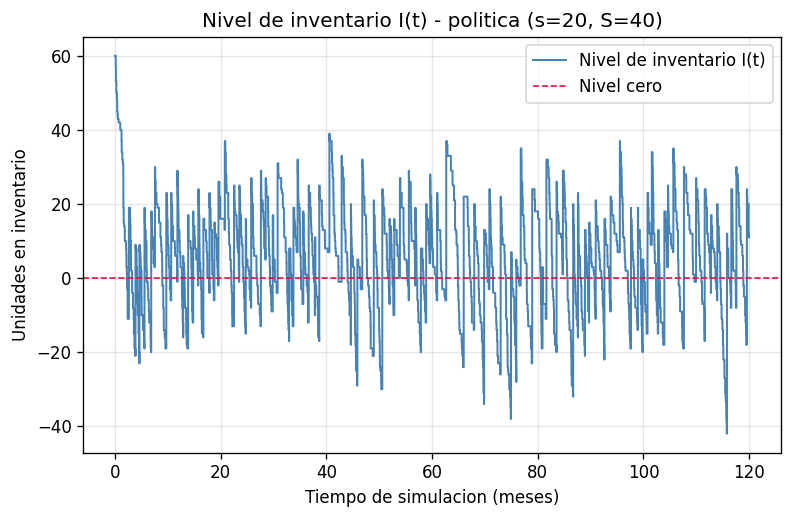
\includegraphics[width=\textwidth]{output/inventario_nivel.png}
  \caption{Evoluci\'on del nivel de inventario $I(t)$.}
  \label{fig:nivel}
\end{subfigure}
\begin{subfigure}{0.48\textwidth}
  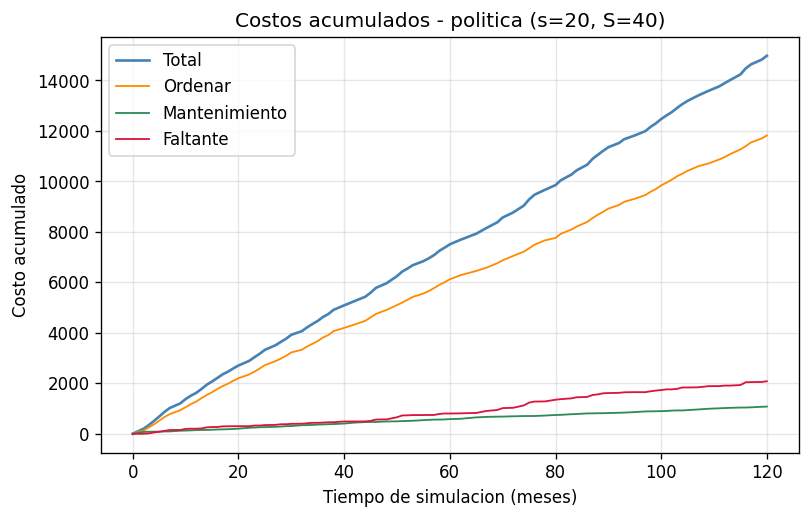
\includegraphics[width=\textwidth]{output/inventario_costos_acumulados.png}
  \caption{Costos acumulados vs.\ tiempo.}
  \label{fig:acumulados}
\end{subfigure}
\\[0.5em]
\begin{subfigure}{0.48\textwidth}
  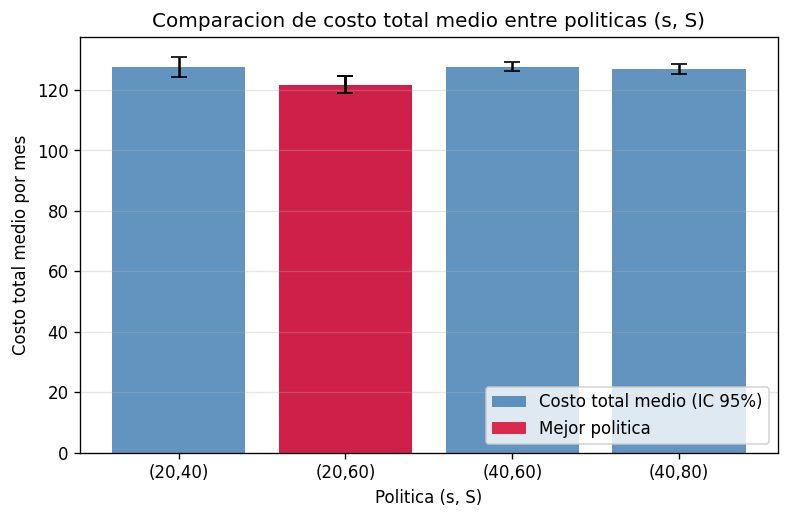
\includegraphics[width=\textwidth]{output/inventario_comparacion_total.png}
  \caption{Costo total por pol\'itica (IC 95\%).}
  \label{fig:comparacion}
\end{subfigure}
\begin{subfigure}{0.48\textwidth}
  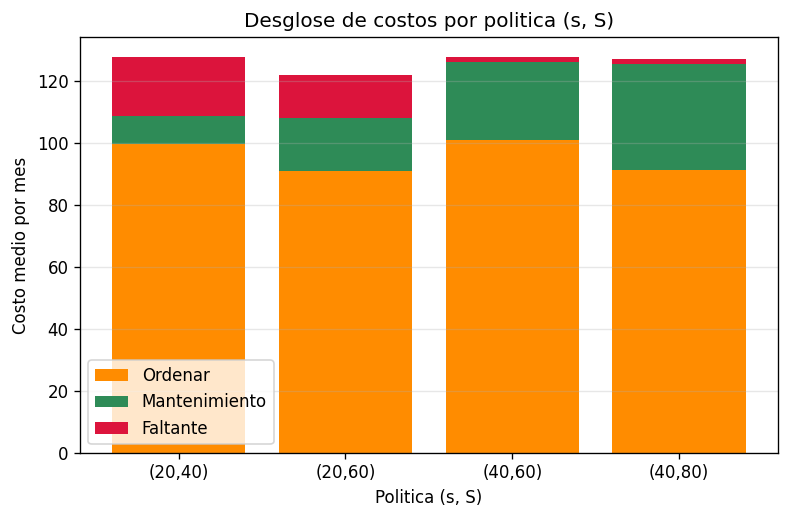
\includegraphics[width=\textwidth]{output/inventario_desglose_costos.png}
  \caption{Desglose de costos por pol\'itica.}
  \label{fig:desglose}
\end{subfigure}
\caption{Resultados de la simulaci\'on. (a) El nivel de inventario $I(t)$
evoluciona en forma escalonada: baja con cada demanda y sube de golpe al
recibirse una orden; la l\'inea del cero separa el inventario positivo (zona de
\emph{holding}) del backlog negativo (zona de \emph{shortage}). (b) Los costos
acumulados crecen mon\'otonamente a lo largo de los $120$ meses. (c) Comparaci\'on
del costo total mensual de las cuatro pol\'iticas con sus barras de error al
$95\%$; la mejor pol\'itica $(20, 60)$ aparece resaltada. (d) Barras apiladas
del desglose ordenar / mantenimiento / faltante de cada pol\'itica, que
visualiza el trade-off entre los tres rubros.}
\label{fig:resultados}
\end{figure}

\subsection{Comparaci\'on de las tres fuentes}

El enunciado del TP exige contrastar TRES fuentes de datos para validar el
modelo: la referencia anal\'itica aproximada, la simulaci\'on en Python y un
modelo equivalente construido en AnyLogic. La Tabla~\ref{tab:fuentes} re\'une las
tres columnas para la pol\'itica recomendada $(20, 60)$. El modelo en AnyLogic se
corri\'o por $120$ meses y los costos acumulados se promediaron mensualmente.

\begin{table}[H]
\centering
\small
\begin{tabular}{lrrr}
\toprule
\textbf{Medida (pol\'itica $(20, 60)$)} & \textbf{Ref.\ anal\'itica}
& \textbf{Python (sim.)} & \textbf{AnyLogic} \\
\midrule
Demanda media (u/mes) & $25{,}00$           & $25{,}00$           & $25{,}00$ \\
Costo de ordenar      & $\approx 90$        & $90{,}88$           & $92{,}36$ \\
Costo de mantenimiento& sin f\'ormula cerrada & $17{,}10$         & $16{,}57$ \\
Costo de faltante     & sin f\'ormula cerrada & $13{,}73$         & $17{,}19$ \\
Costo total mensual   & ---                 & $121{,}71$          & $126{,}12$ \\
\bottomrule
\end{tabular}
\caption{Contraste de las tres fuentes de datos para la pol\'itica $(20, 60)$.
La referencia anal\'itica solo es exacta para la demanda media; el holding y el
shortage no tienen f\'ormula cerrada (ver Secci\'on 2.5). La columna de AnyLogic
corresponde al promedio mensual de una corrida de $120$ meses en AnyLogic PLE.}
\label{tab:fuentes}
\end{table}

\section{Discusi\'on}

\textbf{El trade-off entre los tres costos.} La Tabla~\ref{tab:resultados}
ilustra con claridad el compromiso central del modelo. Subir el nivel objetivo
$S$ eleva el inventario promedio y por lo tanto el costo de mantenimiento: al
pasar de $(20, 40)$ a $(20, 60)$ el holding sube de $8{,}84$ a $17{,}10$, y de
$(40, 60)$ a $(40, 80)$ sube de $25{,}39$ a $34{,}16$. En sentido inverso,
subir el umbral de reorden $s$ reduce dr\'asticamente el faltante: pasar de
$s = 20$ a $s = 40$ (manteniendo la brecha) lleva el shortage de $19{,}20$ a
apenas $\approx 1{,}6$, porque se ordena antes de quedarse sin stock.

\textbf{Por qu\'e gana $(20, 60)$.} La pol\'itica recomendada equilibra ambos
efectos. Un $S$ alto ($60$) implica \'ordenes m\'as grandes y por lo tanto menos
frecuentes, lo que reduce el costo de ordenar (de hecho $(20, 60)$ y $(40, 80)$,
las de mayor $S$, son las de menor costo de ordenar, $90{,}88$ y $91{,}17$). Un
umbral de reorden $s$ moderado ($20$) mantiene el faltante en un nivel
aceptable ($13{,}73$) sin necesidad de cargar con el exceso de stock que
implican las pol\'iticas de $s = 40$. La combinaci\'on de \'ordenes poco
frecuentes y faltante controlado es lo que minimiza el total.

\textbf{Superficie de costo plana.} Un hallazgo notable es que las cuatro
pol\'iticas producen costos totales muy parecidos, todos en la banda
$121$--$128$. Esto indica que la superficie de costo es relativamente
\emph{plana} alrededor del \'optimo: peque\~nos cambios en $(s, S)$ mueven poco
el costo total, porque lo que una pol\'itica ahorra en un rubro tiende a
gastarlo en otro. Es un comportamiento t\'ipico de estos modelos de inventario y
explica por qu\'e la diferencia entre la mejor ($121{,}71$) y la peor
($127{,}70$) pol\'itica es de apenas un $5\%$.

\textbf{Variabilidad entre r\'eplicas.} Los intervalos de confianza al $95\%$
de la Tabla~\ref{tab:resultados} muestran que la incertidumbre estad\'istica
no es despreciable frente a las diferencias entre pol\'iticas. Por ejemplo, el
IC del costo total de $(20, 60)$ ($\pm 2{,}79$) se solapa parcialmente con el de
$(40, 80)$ ($\pm 1{,}75$). Esto refuerza la observaci\'on de la superficie plana
y sugiere que, para distinguir pol\'iticas tan cercanas con mayor confianza,
convendr\'ia aumentar el n\'umero de r\'eplicas. A\'un as\'i, $(20, 60)$ es
consistentemente la de menor media.

\section{Conclusiones}

\begin{enumerate}
  \item La pol\'itica $(20, 60)$ minimiza el costo total mensual ($121{,}71$,
    con IC 95\% $[\,118{,}92\,;\,124{,}50\,]$) entre las cuatro evaluadas, y es
    la recomendada para este sistema.
  \item El modelo simulado reproduce fielmente el comportamiento esperado del
    ejemplo de inventario $(s, S)$ del cap\'itulo 1.5 de Law: demanda media de
    $25$ u/mes, evoluci\'on escalonada de $I(t)$ con backlog, y el trade-off
    caracter\'istico entre ordenar, mantener y faltar.
  \item Los costos est\'an equilibrados entre s\'i y la superficie de costo es
    plana alrededor del \'optimo (totales en la banda $121$--$128$): la
    pol\'itica acertada reparte el gasto entre los tres rubros en lugar de
    minimizar uno solo.
  \item Ante la ausencia de una f\'ormula cerrada exacta para el modelo
    $(s, S)$ con backlog, la simulaci\'on es la fuente confiable del valor
    esperado; la referencia anal\'itica solo sirve como verificaci\'on del
    orden de magnitud (demanda media).
  \item La comparaci\'on de las tres fuentes (anal\'itica, Python, AnyLogic)
    para la pol\'itica $(20, 60)$ arroja valores consistentes en torno a los
    $\$121-\$126$ mensuales, lo que consolida la validez de la simulaci\'on 
    como herramienta de decisi\'on cuando la teor\'ia exacta no es alcanzable.
\end{enumerate}

\begin{thebibliography}{9}

\bibitem{law}
Law, A. M. (2014). \emph{Simulation Modeling and Analysis}
(5\textsuperscript{a} ed.). McGraw-Hill. (Cap\'itulo 1.5: modelo de inventario
de revisi\'on peri\'odica con pol\'itica $(s, S)$).

\bibitem{naylor}
Naylor, T. H. (1982). \emph{T\'ecnicas de simulaci\'on en computadoras}
(cap\'itulo 4: Generaci\'on de valores de las variables estoc\'asticas).
Limusa.

\bibitem{matplotlib}
Hunter, J. D. (2007). Matplotlib: A 2D Graphics Environment.
\emph{Computing in Science \& Engineering}, 9(3), 90-95.

\bibitem{python}
Van Rossum, G., \& Drake, F. L. (2009). \emph{Python 3 Reference Manual}.
CreateSpace.

\end{thebibliography}

\end{document}
